\subsection{Results}\label{sec:m4:results}
    ~\cref{fig:m4:angular_power_spectrum} shows the angular power spectrum as function of photon multipole $l$. The blue drawn line is the main power spectrum, while the dotted lines are the four constituents of the power spectrum that arise from the source function in ~\cref{eq:m3:theory:source_function}. The red lines are observations taken from ~\cite{Planck2020}, and the turquoise shade shows the theoretical cosmic variance as given in ~\cref{eq:m4:theory:cosmic_variance}. As expected, since we ignore both polarisation and neutrinos there is a discrepancy between the observed values and the theoretical prediction. This is most prominent for larger $l$-s where the observational constraints are low due to high statistical accuracy. In discussing this results, we will focus on the three main parts of the plots, namely the \textit{Sachs-Wolfe plateau} for low $l$-s, the \textit{acoustic oscillations} for intermediate $l$-s and the \textit{diffusion damping} for high $l$-s. Lastly we discuss the matter power spectrum in, where we have obtained the observational data from ~\cite{Chabanier_2019} and ~\cite{Hlozek_2012}.
    \begin{figure}
        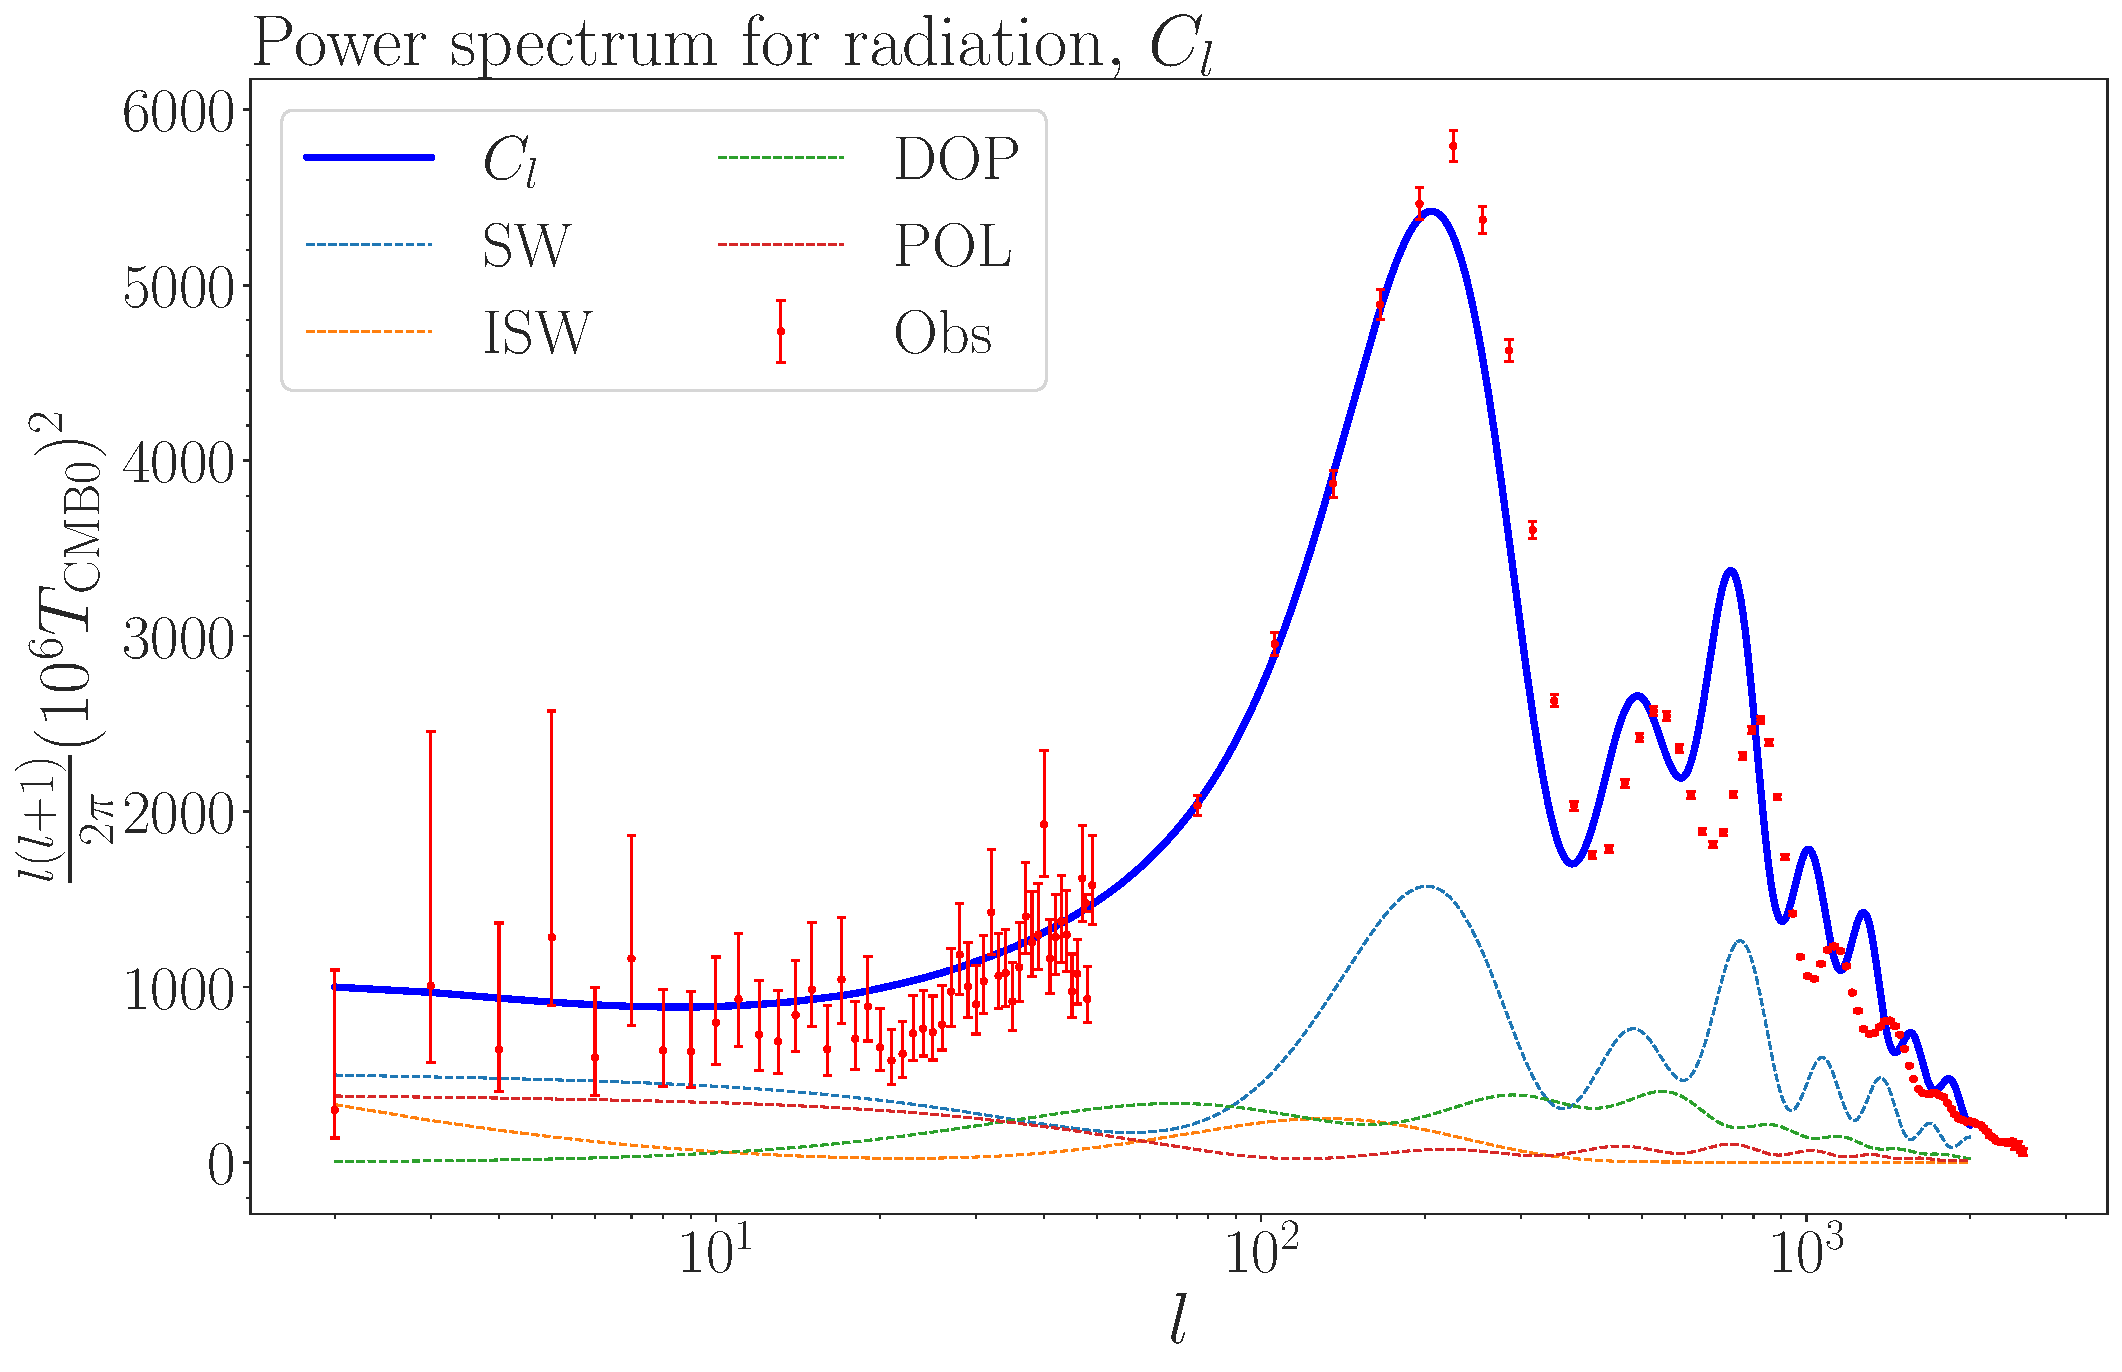
\includegraphics[width=\linewidth]{power_spectrum.pdf}
        \caption{Angular power spectrum as function of photon multipole $l$. The blue line shows the angular power spectrum itself with the intrinsic cosmic variance overplotted in turquoise. The dotted lines are the individual effect of the different constituents of the source function. The red error bars are observational constraints.}
        \label{fig:m4:angular_power_spectrum}
    \end{figure}
    \subsubsection{The Sachs-Wolfe plateau}
        The Sachs-Wolfe plateau is the part of the angular power spectrum that appear fairly flat for low $l$, i.e. large scales, hence it names. These large scale represent modes that had not yet entered the horison at the time of recombination. According to the Sachs-Wolfe (SW) term in the source function in ~\cref{eq:m3:theory:source_function}, the major contribution to the power spectrum are the temperature anisotropies present at the last scattering surface. This is the main contributor to the transfer function and thus the power spectrum itself. These effects are described by the photon monopole, and the value of the gravitational perturbation, $\Psi$, whose main effect slowed the photons down through gravitational redshift.\footnote{Plus a small quadrupole correction.} For large scales, that have not yet entered the horison at the time of last scattering, the fluctuation to the gravitational perturbation have not yet been affected by causal physics. As a result, they closely resemble the initial perturbations induced by inflation. 

        Thus, the Sachs-Wolfe plateau may be understood as a tracer of the primordial power spectrum. If we continue to assume this take the form of a Harrison-Zel'dovich spectrum parametrised by the amplitdue $A_s$ and spectral index $n_s$ we are able to estimate the former by considering the amplitude of the Sachs-Wolfe plateau, and the latter by its shape. $n_s=1$ would generate a flat primordial power spectrum, whereas $n_s>1$ would give emphasis to small scales and vice versa. 

        We also take note of the large cosmic variance in this region. As already explained, this is and intrinsic feature of the angular power spectrum when comparing to observations, as we only have one universe to make observations in. The observational constraints are also significantly larger in this region. As is to be expected. 

        In figure ~\cref{fig:m4:angular_power_spectrum} we also see some contribution from the integrated Sachs-Wolfe (ISW) term, which occur due to changes in the gravitational potentials. Most prominent in the discussion of the Sachs-Wolfe plateau is the late-time ISW which occur around matter-dark-energy equality. These effects can be seen for the largest scales, as they happened quite recently, and contributes to the minor deviations away from a straight line for the Sachs-Wolfe plateau.
        
        There is also an increasing contribution of the Doppler term, which correspond to the peculiar velocity of matter (and our peculiar velocity relative to the CMB-frame). The Sachs-Wolfe plateau indicate the existence of large scale structures in the Universe 

    \subsubsection{Acoustic oscillations}

    \subsubsection{The damping tail}


    \subsubsection{The matter power spectrum}
    
    \begin{figure}
        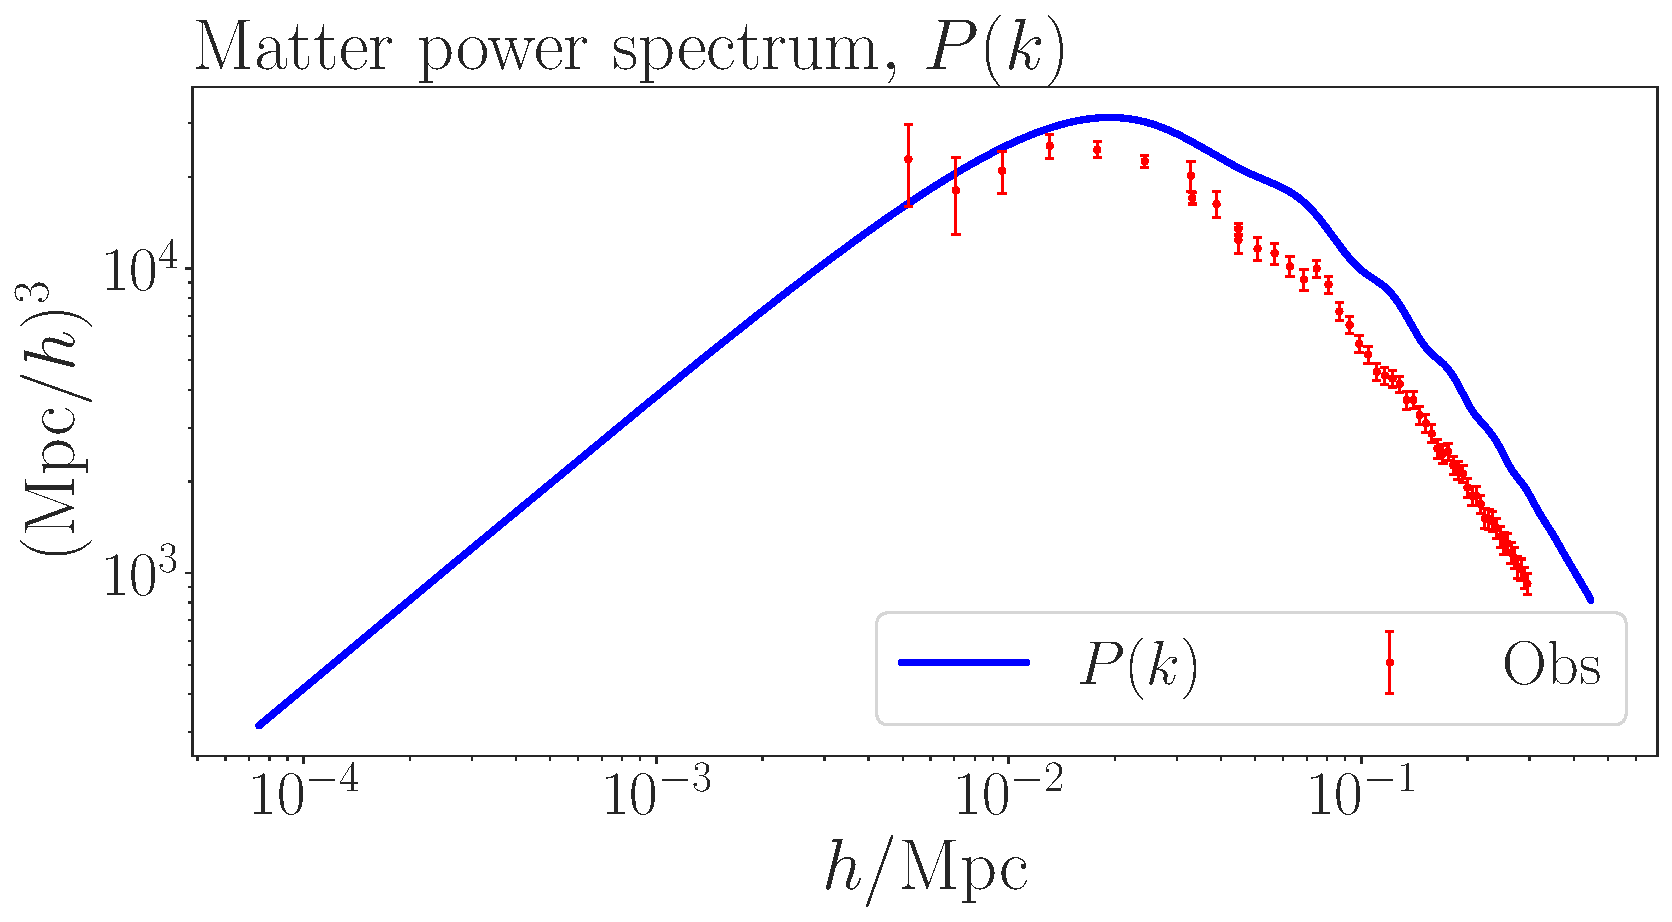
\includegraphics[width=\linewidth]{matter_power_spectrum.pdf}
        \caption{Matter power spectrum as function of wavenumber $k$. The violet dotted line the equality scale, which is the wavenumber that correspond to the mode entering the horison at the time of radiation-matter equality. The red error bars are observational constraints.}
        \label{fig:m4:matter_power_spectrum}
    \end{figure}